\documentclass[12pt]{article}

\usepackage[utf8]{inputenc}
\usepackage[T1]{fontenc}
\usepackage[brazil]{babel}
\usepackage{cancel}
\usepackage{geometry}
\geometry{margin=2.5cm}
\usepackage{setspace}
\onehalfspacing

\usepackage{amsmath, amssymb, amsthm}
\usepackage{mathtools}

\numberwithin{equation}{section}

\theoremstyle{plain}
\newtheorem{theorem}{Teorema}[section]
\newtheorem{proposition}[theorem]{Proposição}
\newtheorem{lemma}[theorem]{Lema}
\newtheorem{corollary}[theorem]{Corolário}

\theoremstyle{definition}
\newtheorem{definition}[theorem]{Definição}
\newtheorem{example}[theorem]{Exemplo}
\newtheorem{exercise}{Exercício}

\theoremstyle{remark}
\newtheorem*{remark}{Observação}

\usepackage{hyperref}
\usepackage{csquotes}

\usepackage[
    backend=biber,
    style=abnt,
    style=authoryear,
    maxcitenames=3
]{biblatex}

\addbibresource{../Microeconomics.bib}


\newcommand{\R}{\mathbb{R}}
\newcommand{\pref}{\succeq}
\newcommand{\strictpref}{\succ}
\newcommand{\indiff}{\sim}

% ------------------------------------------------
% Title (fill manually)
% ------------------------------------------------
\title{Lista 5 --- Teoria Microeconômica (PPGE-UFF)}
\author{Professor: Fábio Waltenberg\thanks{\href{mailto:fdwaltenberg@id.uff.br}{fdwaltenberg@id.uff.br}} \\Monitor: Nicholas Funari Voltani\thanks{\href{mailto:nicholasvoltani@gmail.com}{nicholasvoltani@gmail.com}}}
\date{}

\begin{document}

\maketitle

\hypertarget{conceitos-introdutuxf3rios}{%
\section{Conceitos introdutórios}\label{conceitos-introdutuxf3rios}}

\hypertarget{teoria-da-firma}{%
\subsection{Teoria da firma}\label{teoria-da-firma}}

A teoria da produção em Microeconomia consiste em tratar firmas como ``caixas pretas'' que tomam certos insumos como \textit{inputs} e produzem certos bens como \textit{outputs}. As possibilidades que uma dada firma possui no que tange às proporções de \textit{inputs} para certas quantidades de \textit{outputs} podem ser representadas no que se chama de \textit{conjunto de produção}.

\begin{definition}
Um \textit{conjunto de produção} \(Y\) de uma dada firma é o conjunto
\(Y \subseteq \mathbb{R}^{L}\), em que cada
\(Y \ni y = (y_{1}, \dots, y_n)\) descreve uma possível configuração de
produção, em que \(y_{i}<0\) é um \textit{input} \(y_{i}>0\) é um
\textit{output}.

Em geral, diz-se que qualquer \(y_{i}\) é um ``\textit{netput}''.
\end{definition}

Note-se que, a depender do conjunto de produção \(Y\), pode ser possível que haja ``desperdício'' de inputs, i.e. uma mesma produção de outputs pode demandar mais do que a quantidade ``ótima'' de inputs, ou, por outro lado, uma quantidade de inputs pode produzir uma quantidade ``não-ótima'' de outputs.

\begin{definition}
\parencite[, p. 132]{Mas-Colell1995} Os \textit{retornos de escala} de
um conjunto de produção \(Y\) dizem respeito à \textit{viabilidade} de
aumentar/diminuir a escala de algum plano de produção viável
\(y \in Y\).

As definições são: 
\begin{enumerate}
  \item Retornos \textit{não-crescentes} de escala: para
quaisquer escalares \(\alpha \in [0,1]\) e \(y\in Y\), tem-se que
\(\alpha y \in Y\). Ou seja, se \(y\) é um plano de produção factível,
ele pode ser realizado em menor escala, mas \textit{nada garante} que ele
o será em maior escala.
  \item Retornos
\textit{não-decrescentes} de escala: para quaisquer escalares
\(\alpha \geq 1\) e \(y \in Y\), tem-se que \(\alpha y \in Y\). Ou seja,
se \(y\) é um plano de produção factível, então ele pode ser realizado
em maior escala, mas não necessariamente ele pode ser \textit{scaled
down}.
  \item Retornos \textit{constantes} de escala: são não-decrescentes e
não-crescentes em escala. Portanto, para todo escalar \(\alpha \geq 0\)
e \(y \in Y\), tem-se que \(\alpha y \in Y\).
\end{enumerate}

Pode-se visualizar estes conjuntos da seguinte forma:

\begin{figure}[h!]
  \centering
  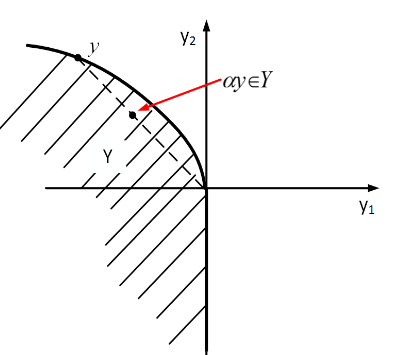
\includegraphics[width=0.45\linewidth]{images/Pasted image 20260521124131.png}
  \caption{Conjunto de produção com retornos \textit{não-crescentes} de escala. Fonte: \href{https://felixmunozgarcia.com/wp-content/uploads/2018/02/chapter-4-production-theory.pdf}{felixmunozgarcia.com/wp-content/uploads/2018/02/chapter-4-production-theory.pdf}.}
\end{figure}


\begin{figure}[h!]
  \centering
  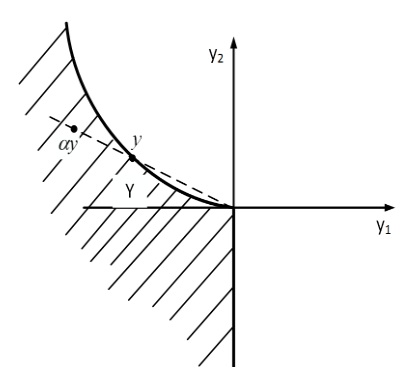
\includegraphics[width=0.45\linewidth]{images/Pasted image 20260521124214.png}
  \caption{Conjunto de produção com retornos de escala \textit{não-decrescentes}. Fonte: \href{https://felixmunozgarcia.com/wp-content/uploads/2018/02/chapter-4-production-theory.pdf}{felixmunozgarcia.com/wp-content/uploads/2018/02/chapter-4-production-theory.pdf}.}
\end{figure}


\begin{figure}[h!]
  \centering
  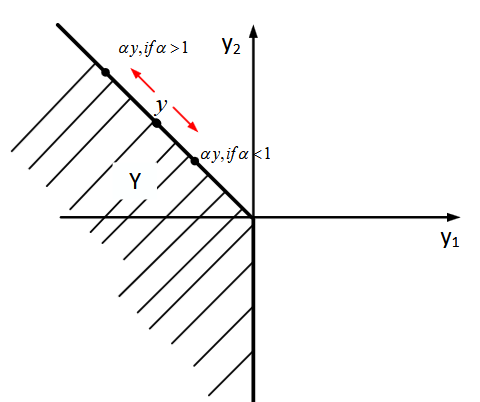
\includegraphics[width=0.45\linewidth]{images/Pasted image 20260521124319.png}
  \caption{Conjunto de produção com retornos de escala \textit{constantes}. Note que ele está no ``meio termo'' entre não-crescente e
não-decrescente, ou melhor, é ambos ao mesmo tempo. Fonte: \href{https://felixmunozgarcia.com/wp-content/uploads/2018/02/chapter-4-production-theory.pdf}{felixmunozgarcia.com/wp-content/uploads/2018/02/chapter-4-production-theory.pdf}.}
\end{figure}
\end{definition}

O mais comum, porém, é de se falar de processos que tomam \(n\) inputs \(z \in \mathbb{R}^{n}\) e produzem somente \(1\) output \(y \in \mathbb{R}_{+}\). Não só isso, é comum também falar-se de \textit{funções de produção} \(f(z) \in \mathbb{R}\) que descrevem processos \textit{ótimos} de produção.

\begin{definition}
Uma função \(f: \mathbb{R}^{n} \to \mathbb{R}_{+}\) é chamada de
\textit{função de produção} se ela descreve um processo de produção
``ótimo'' em um conjunto de produção \(Y \subseteq \mathbb{R}^{n+1}\).
Ou seja, para cada processo de produção
\((z_{1}, \dots, z_{n}, y) \in Y\), tem-se que
\[
f(z) \geq y
\]

Ou seja, o valor \(f(z)\) é o output ótimo que esta firma consegue
produzir a partir destes inputs \(z_{1},\dots,z_{n}\). Isso não quer
dizer que \(f(z)\) é o \textit{único output} possível de se obter com
inputs \(z\) --- pois sempre é possível se produzir \textit{menos
eficientemente}, p.~ex. com algum processo mais desorganizado ---, e sim
\(f(z)\) é o maior output possível de se obter através dos inputs \(z\),
ou, visto de outra forma, é o output que é obtido através do processo
\textit{mais eficiente possível} (com os inputs \(z\)).
\end{definition}

O problema da firma possui um paralelo com o problema do consumidor, consistindo em dois problemas duais: a firma pode buscar \textit{minimizar seu custo de produção}, assim como pode buscar \textit{maximizar seu lucro}. Tais problemas são passíveis de ser descritos pelo formalismo acima.

É mais usual falar sobre a minimização do custo \(\sum \limits_{i=1}^{n} w_{i}z_{i}\) --- em que \(w_{i}\) é o custo do input \(i\), consumido em \(z_{i} \in \mathbb{R}\) ``unidades'' neste processo específico --- para a produção de uma dada quantidade \(\bar{q} \in \mathbb{R}\) de output, com alguma função de produção \(f(z_{1},\dots,z_{n}) \in \mathbb{R}\), e que será vendida a preço \(p\) por unidade produzida. Ou seja, usualmente fala-se do problema de \textit{minimização do custo}.

\textbf{Um comentário sobre notação}: Quando se fala sobre netputs, costuma-se empregar $p_i$ como os preços de todos estes elementos da produção. Contudo, conforme notação usual, empregaremos \(w_{i}\) como o \textit{custo do insumo} \(i\) --- quando for cabível discerni-lo do produto, especialmente em processos de produção de somente um produto $q$ ---, análogo ao \textbf{w}age/preço da força de trabalho, e \(p_{j}\) como o \textit{preço do produto} \(j\). Não confundir estes \(w\)'s com ``restrições orçamentárias''!

\begin{definition}
O problema de minimização do custo de uma firma com conjunto de produção
\(Y \in \mathbb{R}^{n+1}\) e função de produção
\(f: \mathbb{R}^{n} \to \mathbb{R}_{+}\), dados os preços de seus
insumos \(w \in \mathbb{R}^{n}\), consiste no problema
\[
\min\limits_{z \in \mathbb{R}^{n}} \sum \limits_{i=1}^{n} p_{i}z_{i \,\,\,} \text{  t. q. } \, f(z) \geq q
\]
I.e. minimizar o custo com o qual pode-se produzir \textit{no mínimo}
\(q\) unidades de output; ou seja, ``aproveita-se ao máximo'' os insumos
dados. Denote-se os valores ótimos dessa minimização como \(z_{i}^*\).

As quantidades ótimas dos inputs empregados sob este problema (de
minimização de custo) são denominadas de \textit{demandas condicionais}
\(H^{i}(w,q)\) deste processo \parencite[, p. 23]{Cowell2004}, denotadas
como
\[
H^{i}(w, q) \coloneqq z^{*}_{i}
\]

Os valores da função minimizada neste problema compõem a \textit{função
custo} desta firma:
\[
C(w,q) \coloneqq \sum \limits_{i=1}^{n} p_{i} z^{*}_{i} = \sum \limits_{i=1}^{n}p_{i} H^{i}(w, q)
\]
Como Cowell o coloca, a função custo descreve ``o investimento
{[}\textit{outlay}{]} mínimo que a firma exige para adquirir os
insumos'', dados os preços dos insumos \(w\) e o nível de produção \(q\)
\parencite[, p. 23]{Cowell2004}.

Há um claro análogo com a teoria do consumidor, em que a \textit{função
dispêndio}
\[
e(p, \bar{u}) = \sum \limits_{i=1}^{n} p_{i} x_{i}^{*}
\]
é a \textit{restrição orçamentária mínima} com a qual alcança-se um
nível de utilidade \(\bar{u}\) sob preços \(p\) dos bens consumidos
\(x_{i}^{*}\)\footnote{Demandas estas que, sob o problema de minimização
  da restrição orçamentária, são Demandas Hicksianas.} em uma cesta.
\end{definition}

Por outro lado, o formalismo mais geral de conjuntos de produção, em que inputs são ``negativos'' e outputs são ``positivos'', permite uma descrição mais elegante do problema de \textit{maximização do lucro}.

\begin{definition}
O problema de maximização do lucro de uma firma que tenha um conjunto de
produção \(Y \in \mathbb{R}^{n}\) pode ser escrito, no caso geral, como
\[
\max\limits_{y \in Y} \sum \limits_{i=1}^{n} p_{i}y_{i}= \max\limits_{y \in Y} \left\{\underbrace{ \sum \limits_{i} p_{i} y_{i} }_{ \underset{(y_{i} > 0)}{\text{Receita } }} - \underbrace{ \sum \limits_{j} p_{j}|y_{j}| }_{ \underset{(y_{j} < 0)}{\text{Custo}}}\right\}
\]

O caso usual, em que empregam-se \(n\) inputs \(z_{1},\dots,z_{n}\) (com
preços \(w_{1},\dots,w_{n}\)) para a produção de um output \(q\) (com
preço \(p\)), escreve-se como
\[
\max\limits_{x_{i}, q \,\in \mathbb{R}} \left\{pq - \sum \limits_{i}w_{i}z_{i}\right\}
\]

Supondo que a firma tenha uma função de produção
\(f(x_{1},\dots,x_{n}) \equiv f(x)\), o problema se escreve\footnote{Pois,
  lembrando da definição de função de produção, \(f(z)\) é a quantidade
  ótima que se pode obter de \(z_{1},\dots,z_{n}\). É por isso que o
  problema restringe-se a buscar otimizar somente \(z\), invés de \(z\)
  e \(q\).}
\[
\max\limits_{z_{i} \in \mathbb{R}} \left\{pf(z) - \sum \limits_{i}w_{i}z_{i}\right\}
\]

\end{definition}







\hypertarget{exercuxedcios}{%
\section{Exercícios}\label{exercuxedcios}}

\begin{exercise}
\parencite[, pp. 135-6]{Mas-Colell1995} Seja \(Y\) um conjunto de
produção com retornos de escala \textit{não-decrescentes}. Ou seja,
\[
\forall y \in Y, \forall \alpha\geq 1: \alpha y \in Y
\]

Prove que, dados preços \(p\) --- de insumos e de produtos ---, o
lucro\footnote{Lembrando que, num conjunto de produção \(Y\), insumos
  são valores negativos, e produtos são valores positivos.}
\[\pi(p) \coloneqq \max\limits_{y \in Y} p \cdot y\] 
desta firma ou tende a \(\infty\), ou \(\pi(p) \leq 0\).

(Note que este caso não é sustentável na realidade. O que \textit{pode} acontecer é que um certo processo de produção tenha \textit{localmente} retornos de escala não-decrescentes, mas que, a escalas de produção maiores, ele tenha \textit{rendimentos marginais decrescentes}.)
\end{exercise}

\begin{exercise}
Suponha que \(f: \mathbb{R}^{L-1} \to \mathbb{R}\) seja a função de
produção de um único produto, e seja \(Y \subseteq \mathbb{R}^L\) o
respectivo conjunto de produção.

Mostre que \(Y\) satisfaz retornos constantes de escala se, e somente
se, \(f\) é homogênea de grau \(1\).
\end{exercise}

\begin{exercise}
Para uma firma com função de produção
\[
f(K, L) = K^{\alpha}L^{\beta}
\]
em que \(K\) tem ``preço'' \(r\) (produtividade marginal do capital/taxa
real de juros) e \(L\) tem ``preço'' \(w\) (produtividade marginal do
trabalho/salário real).

Resolva o problema de minimização de custo no curto prazo (\(K=\bar{K}\)
fixo, \(L\) variável) e longo prazo (\(K,L\) variáveis), obtendo as
respectivas demandas condicionais \(K^{*}(r,w,q)\) e \(L^{*}(r,w,q)\)

\begin{align*}
\text{Curto prazo: }&  \begin{cases}
K^{*} = \bar{K} \\
L^{*}(w,r,q;\bar{K}) = \left( \frac{q}{\bar{K}^{\alpha}} \right)^{1/\beta}
\end{cases} \\
\text{Longo prazo: }& \begin{cases}
K^{*}(w,r,q) = q^{1/\alpha+\beta} \left( \frac{w}{r} \frac{\alpha}{\beta} \right)^{\beta/\alpha+\beta} \\
L^{*}(w,r,q) = q^{1/\alpha+\beta} \left( \frac{r}{w} \frac{\beta}{\alpha} \right)^{\alpha/\alpha+\beta}
\end{cases}
\end{align*}

e respectivas funções custo:\footnote{[Nota do Nicholas] Citando o honorável
  professor do IFUSP João Carlos Alves Barata --- autor das
  enciclopédicas
  \href{https://denebola.if.usp.br/~jbarata/Notas_de_aula/capitulos.html}{Notas
  (de Física Matemática) do Barata} ---, é bom ``fazer estas contas ao
  menos uma vez na vida'' --- e depois meramente usar os resultados que
  outros já tiveram a dor de cabeça de calcular!}

\begin{align*}
&\text{Curto prazo: } C(w,r,q; \bar{K}) = r \bar{K} + w \left( \frac{q}{\bar{K}^{\alpha}}\right)^{1/\beta} \\
&\text{Longo prazo: } C(w, r, q) = q^{1/\alpha+\beta}  \left[ r^{\alpha} \left(w \frac{\alpha}{\beta} \right)^{\beta/\alpha+\beta}
+ w^{\beta} \left( r \frac{\beta}{\alpha} \right)^{\alpha/\alpha+\beta} \right]
\end{align*}
\end{exercise}

\begin{exercise}
Considere um indivíduo com utilidade quase-linear
\(u(x, m) = \phi(x) + m\),. Assuma que há uma firma com função de custos
\(C(q) = \sigma q\) (\(\sigma>0\)), e que este indivíduo recebe todos os
lucros desta firma. Assuma que a dotação inicial do numerário é
\(\omega_{m}>0\) e a do bem \(x\) é \(\omega_{x}=0\).

Assume-se que tanto a firma quanto o consumidor são tomadores de preço: \(x\) tem preço \(p\), e \(m\) tem preço \(1\)\footnote{I.e.
  \(m\) é assumido como numerário.}. Note que o preço \(p\) do bem \(x\)
conta para o consumidor (i.e. é um dispêndio) e para a firma (i.e.~conta
para sua receita).

\begin{enumerate}
\item
  Derive as condições de primeira ordem do consumidor e da firma, para
  \(\phi(x)\) genérica. Como a condição fica para
  \(\phi(x)=\alpha+\beta \ln x\)?
\item
  Derive o preço de equilíbrio competitivo e o produto do bem \(x\), e a
  quantidade de \(x\) produzido pela firma. Como eles variam conforme
  \(\sigma\), e com relação a \(\alpha,\beta\) do subitem
  acima?\footnote{Exercício de uma lista de um dos monitores prévios
    desta disciplina, Carlos Henrique de C. Júnior.}
\end{enumerate}
\end{exercise}

\hypertarget{resoluuxe7uxf5es}{%
\section{Resoluções}\label{resoluuxe7uxf5es}}
\setcounter{exercise}{0}

\begin{exercise}
Caso haja \textit{algum} processo de produção \(y \in Y\) tal que
\(p \cdot y > 0\), então, pela hipótese de retornos de escala
não-decrescente, este processo pode ser expandido para \(\alpha y\),
gerando um lucro maior. Por hipótese, este processo pode ser extendido
\textit{ad infinitum}; portanto, a função lucro, sendo o \textit{máximo}
de \(p\cdot y\), é ilimitada, i.e.~\(\pi(p)\to \infty\).

O caso oposto, em que \textit{todos} os processos \(y \in Y\) fazem com
que \(p \cdot y \leq 0\), farão com que \(\pi(p) \leq 0\)
inequivocamente.

Portanto, tendo \(Y\) com retornos não-decrescentes de escala,
\(\pi(p) \to \infty\) ou \(\pi(p) \leq 0\).
\end{exercise}

\begin{exercise}
(\(\implies\)) \(Y\) ter retornos constantes de escala quer dizer que
\[
\forall y \in Y, \forall \alpha\geq 0: \alpha y \in Y
\]

Dado algum insumo \(z\), tenhamos, em particular, \(y=(z, f(z))\).
Então, por hipótese, temos que
\(\alpha y=(\alpha z, \alpha f(z)) \in Y\). Porém, por definição,
\(f(z)\) é a quantidade ótima que se pode produzir através de \(z\);
portanto, para \(\alpha z\), vale que
\[
\underbrace{ f(\alpha z) }_{ \text{Qtd. ótima prod. com } \alpha z } \geq\underbrace{ \alpha f(z) }_{ \text{Qtd. retornos cte. escala} }
\]

O mesmo vale fazendo o ``caminho inverso'': tenhamos, em particular,
\(\tilde{y} = (\tilde{z}, f(\tilde{z})) \in Y\), então
\[
\alpha^{-1}\tilde{y} = (\alpha^{-1}\tilde{z}, \alpha^{-1}f(\tilde{z}))
\]
Façamos agora \(\tilde{z}=\alpha z\). Então teremos
\[
y = (z, f(\alpha z)) \in Y \implies \alpha^{-1} y = (z, \alpha^{-1}f(\alpha z)) \in Y
\]

Assim como acima,
\[
f(z)\geq \alpha^{-1}f(\alpha z)  \iff f(\alpha z) \leq \alpha f(z)
\]

Portanto, \(f(\alpha z) = \alpha f(z)\), e \(f\) é homogênea de grau
\(1\).

(\(\impliedby\)) Seja \(\alpha\geq 0\). Então, por hipótese,
\(f(\alpha z)=\alpha f(z)\).

Tenha-se algum \(y = (z, q) \in Y\). Então
\(\alpha y=(\alpha z, \alpha q)\). Em particular, pela definição da
função de produção,
\[
\alpha q\leq f(\alpha z) = \alpha f(z)
\]

Portanto {[}para um conjunto de produção suficientemente
bem-comportado{]}, teremos que, por valer \(\alpha q \leq \alpha f(z)\),
valerá
\[
(\alpha z, \alpha f(z)) \in Y \implies (\alpha z,\alpha q) \in Y
\]

Portanto, \(Y\) terá retornos constantes de escala.
\end{exercise}

\begin{exercise}
\textit{Curto prazo}: Tenha-se \(K = \bar{K}\). Então, é possível isolar
\(L\) através de

\begin{align*}
q = f(\bar{K},L) &= \bar{K}^{\alpha} L^{\beta} \\
\implies L^{*} &= \bar{K}^{\alpha/\beta} q^{1/\beta}
\end{align*}

Não há ``minimização de custo'' aqui, pois o estoque fixo de capital
\(\bar{K}\) e a isoquanta \(f(\bar{K},L) = q\) determinam o nível \(L\)
demandado: despende-se \(L^{*}\) de trabalho para \(\bar{K}\) de
capital, proporção esta ditada pela função de produção \(f\).

A função custo no curto prazo é
\[
C(\bar{K},L^{*}) = \underbrace{ r\bar{K} }_{ \text{Custo fixo } c_{f} } + \underbrace{ w \bar{K}^{\alpha/\beta} q^{1/\beta} }_{ \text{Custo variável } c_{v}(q) }
\]

\textit{Longo prazo}: O problema de minimização do custo \(rK + wL\),
dado um nível de produção \(q=f(K,L) = K^{\alpha}L^{\beta}\), é
resolvido pela otimização do lagrangiano
\[
\mathcal{L}(K, L, \lambda) = rK+wL - \lambda (K^{\alpha}L^{\beta} - q)
\]

A otimização de \(\mathcal{L}\) traz
\[
\begin{cases}
\frac{ \partial \mathcal{L} }{ \partial K } &= 0 \implies r = \alpha \lambda K^{\alpha-1} L^{\beta} \\
 \frac{ \partial \mathcal{L} }{ \partial L } &=0 \implies w = \beta \lambda K^{\alpha}L^{\beta-1} \\
 \frac{ \partial \mathcal{L} }{ \partial \lambda } &=0 \implies q = K^{\alpha}L^{\beta}
\end{cases}
\]

Dividindo a primeira equação pela segunda, temos
\[
L^{*} = \frac{r}{w} \frac{\beta}{\alpha} K^{*}
\]

Substituindo na restrição (terceira equação), temos

\begin{align*}
q &= K^{\alpha}L^{\beta} \\
&= K^{\alpha} \left( \frac{r}{w} \frac{\beta}{\alpha} \right)^{\beta} K^{\beta} \\
\therefore K^{*} &= q^{1/\alpha+\beta} \, \left( \frac{w}{r} \frac{\alpha}{\beta} \right)^{\beta/\alpha+\beta}
\end{align*}

Ressubstituindo na equação de \(L^{*}\), temos

\begin{align*}
L^{*} &= q^{1/\alpha+\beta} \, \left( \frac{r}{w} \frac{\beta}{\alpha}  \right) \left( \frac{w}{r} \frac{\alpha}{\beta} \right)^{\beta/\alpha+\beta} \\
&= q^{1/\alpha+\beta} \, \left( \frac{w}{r} \frac{\alpha}{\beta} \right)^{(-\alpha-\beta)/\alpha+\beta} \left( \frac{w}{r} \frac{\alpha}{\beta} \right)^{\beta/\alpha+\beta} \\
&= q^{1/\alpha+\beta} \left( \frac{w}{r} \frac{\alpha}{\beta} \right)^{-\alpha/\alpha+\beta} \\
\therefore L^{*} &= q^{1/\alpha+\beta} \left( \frac{r}{w} \frac{\beta}{\alpha}  \right)^{\alpha/\alpha+\beta}
\end{align*}

A função custo, sendo \(C(r,w,q) = r K^{*} + w L^{*}\), fica

\begin{align*}
C(r,w,q) &= q^{1/\alpha+\beta} \left( \frac{r^{(\alpha+\cancel{ \beta })/\alpha+\beta}}{r^{\cancel{ \beta }/\alpha+\beta}} \left( w \frac{\alpha}{\beta} \right)^{\beta/\alpha+\beta} + \frac{w^{(\cancel{ \alpha }+\beta)/\alpha+\beta}}{w^{\cancel{ \alpha }/\alpha+\beta}}\left( r \frac{\beta}{\alpha} \right)^{\alpha/\alpha+\beta} \right) \\
&= q^{1/\alpha+\beta} \left( r^{\alpha/\alpha+\beta} \left( w \frac{\alpha}{\beta} \right)^{\beta/\alpha+\beta} + w^{\beta/\alpha+\beta} \left( r \frac{\beta}{\alpha} \right)^{\alpha/\alpha+\beta} \right)
\end{align*}

Note que não há nenhum termo de custo fixo, pois, \textit{no longo
prazo}, mesmo o fator de produção \(K\) também é passível de ser variado
(no que tange à produção de \(q\)).
\end{exercise}

\begin{exercise}
Maximização da utilidade do consumidor \(u(x,m) = \phi(x) + m\), com
restrição orçamentária
\[
p\cdot x+1\cdot m \leq \omega_{m}
\]

Condições de primeira ordem:\footnote{Evitando Kuhn-Tucker, \textit{as
  per usual}\ldots{}}
\[
\begin{cases}
\phi^\prime(x) + \lambda p = 0 \\
1 + \lambda = 0
\end{cases}
\]

Como \(\lambda=-1\), teremos que tem de valer
\[
\phi^\prime(x) = p
\]

Para o caso específico de \(\phi(x) = \alpha+\beta \ln x\), teremos
\[
x^* = \frac{\beta}{p}
\]

Ressubstituindo na restrição orçamentária, teremos que \begin{align*}
m^* &= \omega_{m}-p x^* \\
&= \omega_{m}- \beta
\end{align*}

Maximização do lucro da firma requer a maximização da função lucro
\[
\pi(q) = pq-\sigma q = (p-\sigma)q
\]

Como só teremos que \(\pi\geq 0 \iff p \geq \sigma\); evitando soluções
de canto, requer-se que \(p=\sigma\).

Portanto, quando ambas as soluções valem, teremos (para a \(\phi(x)\)
logarítmica acima)
\[
\begin{cases}
p=\sigma \\
x^*=\frac{\beta}{\sigma} \\
m^* = \omega_{m}-\beta
\end{cases}
\]

\end{exercise}

\printbibliography

\end{document}
